\documentclass{article}
%\usepackage[cyr]{aeguill}
\usepackage[utf8]{inputenc}
\usepackage[T1]{fontenc}
\usepackage[francais]{babel}
\usepackage{amsmath}
\usepackage{fancyhdr}
\usepackage{amsfonts}
\usepackage{makeidx}         
\title{Projet GM4 : Programme de détection de spam}
\usepackage[pdftex]{graphicx}
\author{Jean Prost \and Edouard Gouteux \and Lucas Potin} 
 
\begin{document}
\maketitle
\begin{center}
\begin{figure}[h]
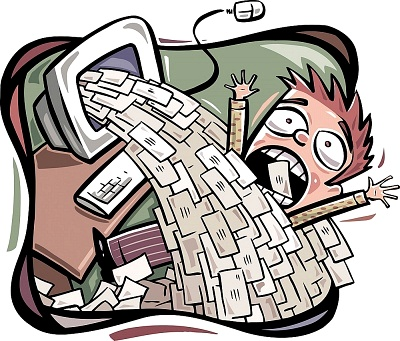
\includegraphics[scale=0.9]{email-spam.jpg}
\end{figure}
\end{center}
\clearpage
\renewcommand{\contentsname}{Sommaire} 
\tableofcontents
\clearpage
 
% une série de blocs comme celui qui suit
\section{Introduction à la méthode}

L'idée principale de la méthode qui va être présentée ici est que l'on peut prédire de manière correct si un mail est un spam ou non, ceci uniquement à l'aide d'une combinaison bayésienne de probabilités de mots présents dans un mail traité. L'idée est de faire ressortir les mots ( ou extraits de code html ) d'un mail qui nous donnent un indice significatif sur la probabilité que ce mail soit un spam ou non, et ceci de manière la plus efficace possible. Cette méthode plutôt simple a déjà fait ses preuves et permet de montrer que les méthodes les plus sophistiquées ne sont parfois pas les plus optimales pour le traitement de problèmes simples tel que la filtration des spams.

\section{Pré-traitement}

\subsection{La phase de pré-traitement d'un corpus ou d'un mail}

Nous allons appliquer notre algorithme sur un texte comprenant uniquement des mots ou expressions traitables, c'est à dire n'ayant pas une taille trop significative ( dans ce cas il y aurait peu de chance que l'expression serve lors du calcul des probabilités, puisque cette expression n’apparaîtrait qu'une seule fois). Nous devons donc effectuer un pré-traitement du texte brut (code html compris ) avant le "vrai" traitement afin "d'épurer" le texte brut de tout ce qui nous est inutile pour le calcul des probabilités de chaque mot. 
Pour se faire, il nous faut extraire les indices les plus significatifs du code html ( par exemple les couleurs très criardes utilisées pour les publicités ) ou encore des termes qui sont redondants dans les spams. Le reste sera supprimé afin de ne garder que le nécessaire pour le calcul du nombre d'occurrence de chaque jeton. 

\subsection{Détail de la phase de pré-traitement}

%%je vais approfondir 
On balaie l'intégralité du texte, y compris les en-têtes, les scripts HTML et JavaScript intégrés, de chaque message de chaque corpus. On considère  que les caractères alphanumériques, les tirets, les apostrophes et les signes en dollars font partie des jetons, et que tout le reste est un séparateur de jetons. On ignore les jetons qui sont tous des chiffres et également les commentaires html, sans même les considérer comme des séparateurs de jetons.

De chaque pré-traitement sur un corpus résulte une table de hachage contenant un ensemble de jetons avec pour chaque jeton le nombre d'apparition dans le corpus.

\section{Phase de traitement principal}

\subsection{Le calcul des probabilités}

%%je vais approfondir
Après avoir trié et répertorié nos jetons, nous obtenons un ensemble de jeton avec leur nombre d'occurrence dans chacun des corpus. Nous pouvons extraire, pour chaque jeton, la probabilité qu'un mail soit un spam sachant que le mail contient ce jeton. On notera :

\begin{itemize}
	\item[S] : l'événement "le mail est un spam"
	\item[$\overline{S}$] : l'événement contraire de S, i.e "le mail n'est pas un spam"
	\item[J] : l'événement "le jeton est contenu dans le mail"
\end{itemize}

La probabilité qu'un mail soit un spam sachant que le mail contient ce jeton, $P(S|J)$,  est alors donnée par la formule :
\begin{equation}
P(S|J)=\frac{P(J|S)}{P(J|\overline{S})+P(J|S)}
\label{PSJ}
\end{equation}
Par ailleurs, le nombre d'occurrence du jeton dans les corpus de spam et de non-spam nous permet de calculer les probabilités $P(J|S)$ (i.e la probabilité que le jeton appartienne à un mail sachant que celui-ci est un spam) et $P(J|\overline{S})$ (i.e la probabilité que le jeton appartienne à un mail sachant que celui n'est pas un spam). En notant $n_{s}$ le nombre d'occurrence du token dans le corpus de spam, et $N_{s}$ le nombre de mail du corpus de spam, On a :
\begin{equation}
P(J|S) = min(1,\frac{n_{s}}{N_{s}})
\end{equation}
\begin{equation}
P(J|\overline{S}) =min(1,\frac{n_{ns}}{N_{ns}})
\end{equation}
Ainsi, l'équation \ref{PSJ} devient :
\begin{equation}
P(S|J) = \frac{min(1,\frac{n_{s}}{N_{s}})}{ min(1,\frac{n_{ns}}{N_{ns}})+min(1,\frac{n_{s}}{N_{s}})}
\end{equation}

\subsection{Données d’entraînements}

Avant de pouvoir appliquer notre algorithme à un mail afin de savoir si c'est un spam ou non et de pouvoir faire des tests avec des échantillons de mails spams et/ou non-spam, 
nous avons besoin de données d'entraînement. Ces données d'entraînement sont nécessaires afin que notre algorithme "apprenne" en quelque sorte à détecter les spams. ( voir partie sur le pré-traitement et sur le calcul des probabilités ) 
Pour obtenir un bon taux de prédiction, nous avons besoin d'un corpus de mail d'apprentissage conséquent. En effet, 4000 mails spam et 4000 non spam serait l'idéal.

\section{La phase de prédiction}

Après avoir effectué les étapes précédentes, nous pouvons commencer à prédire si un mail est un spam ou non à l'aide de notre algorithme. Pour cela, un pré-traitement est déjà appliqué au mail afin d'obtenir la table d’occurrence nécessaire au calcul des probabilités. L'algorithme parcours le mail et répertorie les jetons présents à l'intérieur de celui-ci. Enfin, nous usons des 15 jetons ayant les probabilités les plus significatives à l’intérieur du mail afin de déterminer si oui ou non notre mail est un spam. On note : 
\begin{itemize}
	\item[S] : l'événement "le mail est un spam"
	\item[$\overline{S}$] : l'événement contraire de S, ie "le mail n'est pas un spam"
	\item[Ji] : l'événement "le ième jeton le plus significatif est contenu dans le mail" ($i \in {1,...,15}$)
\end{itemize}
La probabilité que le mail soit un spam sachant que les jetons $j_i$ appartiennent au mail est alors donné par la formule :
\begin{equation}
P(S|J_1,J_2,...,J_15) = \frac{\prod_{i=1}^{15}P(S|Ji)}{\prod_{i=1}^{15}P(S|Ji)+\prod_{i=1}^{15}P(\overline{S}|Ji)}
\end{equation}
\section{Regard critique sur la méthode}

Selon le créateur de cette méthode, il faudrait instaurer un "seuil" de filtrage afin de diminuer le nombre de faux spams (mails qui ne sont pas des spams mais qui sont répertoriés comme tel par l'algorithme). Car en effet, une personne préfère en général recevoir quelque spams dans sa boite mail que de voir un message important finir dans les courriers indésirables. La démarche serait alors d'augmenter la tolérance du filtre en considérant le mail comme spam à partir d'une probabilité calculée de 0.95 au lieu de 0.9 par exemple.\\ 
Avoir un bon algorithme de prédiction de spams peut être dangereux. En effet, si l'algorithme est très performant et que nous lui faisons trop confiance, nous pouvons passer à côté d'un mail important, ce qui présente un problème.\\  Un autre problème  est que la méthode naïve du filtre de Bayes est facilement contournable pour les spammeurs, en effet, ceux-ci font désormais ce que l'on appelle des "good word attacks". cette technique consiste simplement à modifier un message spam en y insérant ou en ajoutant des mots indiquant un courrier électronique légitime. Cette technique contre facilement les techniques de filtration de spam comme celle décrite dans ce rapport.\\  

\clearpage

\section{Modélisation UML}

Les classes java utilisées pour l'implémentation de la méthode : \\
Le pré-traitement des mails/corpus en général nous amène à l'utilisation d'une classe Mail qui vas nous servir pour traduire un mail en un ensemble de jetons.
- Extracteur : classe relative au traitement du texte, contient les méthodes permettant de remplir les différents types de table de hachage. \\
- Predicteur : classe qui sert de support aux méthodes permettant de prédire si un mail est un spam ou non. \\
- Mail : Ensemble de jetons ( les jetons sont traduit par des String en java ici ) il s'agit \\

2 types de Table de Hachage découlant de la classe abstraite java HashMap :\\
- TableOccur : table contenant les mails (Non Spam / Spam).\\
- TableProba : table contenant les probabilités basée sur l'apparition des jetons dans les mails spam/non spam.\\

\subsection{Diagramme de classe}

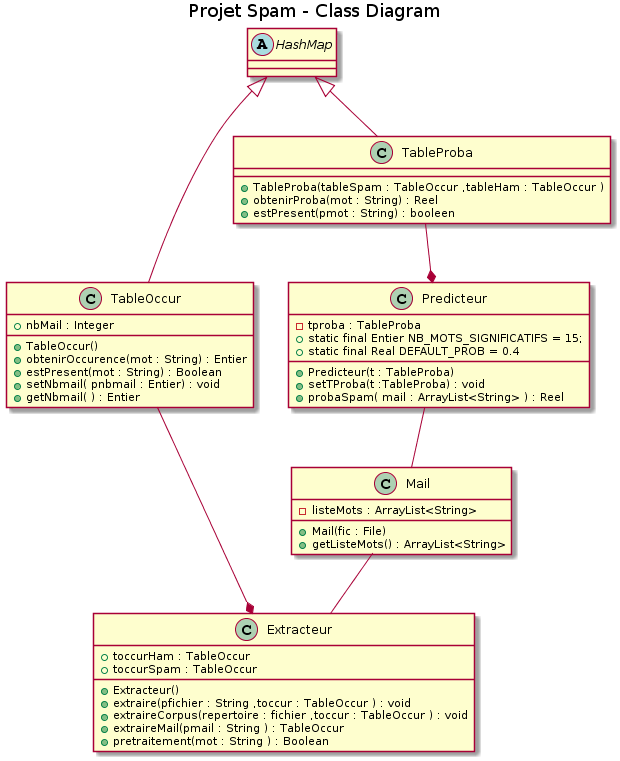
\includegraphics[scale=0.5]{diag_classe.png}

\subsection{Diagramme des cas d'utilisation}
Notre programme java permet à un utilisateur deux choses :\\ Effectuer la phase d'apprentissage du programme en proposant à celui-ci un corpus de spam et un corpus de mails non-spam. Cette phase permettra à l'algorithme de se familiariser avec les données de l'utilisateur. \\
Dans le cas où l'algorithme a déjà effectué la phase d'apprentissage, un utilisateur peut
utiliser l'algorithme afin de prédire si un mail donné ( sous forme de fichier .txt) est un spam ou non.

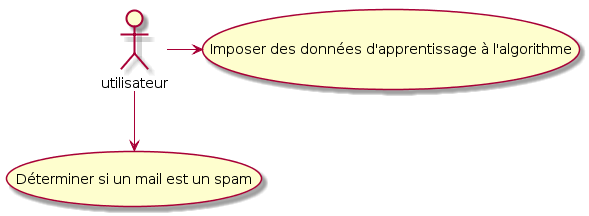
\includegraphics[scale=0.6]{diag_usecase.png}

\subsection{Diagramme de séquence}
On considère la situation où l'utilisateur souhaite connaître la probabilité estimée que son mail soit un spam.

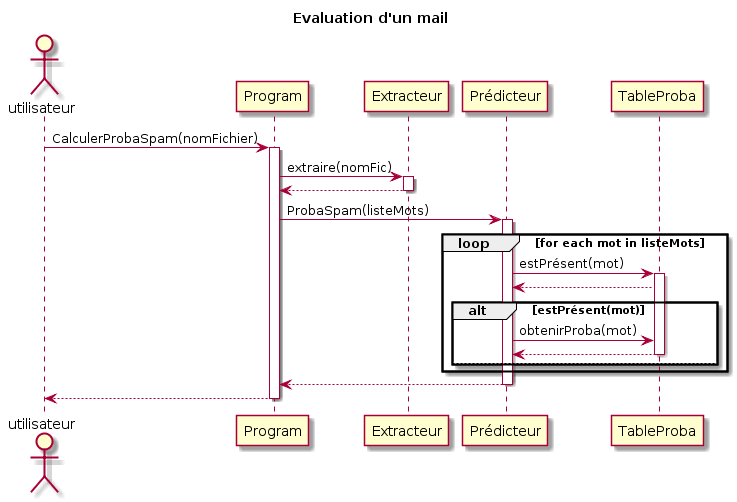
\includegraphics[scale=0.5]{diag_sequence_prediction.png}
\section{Résultats}
\subsection{Nota Bene}
Lors de notre étude , nous avons séparés 2 types de mails : les mails du corpus , qui permettront l'apprentissage et les mails de test , qui vont permettre de sortir des statistiques. Durant toute cette section , le modèle n'apprendra pas des mails des test, qui pourront donc être réutilisés sans fausser le modèle.
De plus , nous listerons ici toutes nos sources ayant permis de récuperer des données :
\begin{itemize}
    \item http://www2.aueb.gr/users/ion/data/enron-spam/
    \item https://spamassassin.apache.org
    \item https://github.com/zrz1996/Spam-Email-Classifier-DataSet
    \item https://plg.uwaterloo.ca/~gvcormac/treccorpus/
\end{itemize}
\subsection{Corpus}
Pour réaliser nos premiers tests, nous avons décidé d'utiliser un corpus de spams en anglais , ceci pour deux raisons : 
\begin{itemize}
    \item Il nous était tout d'abord plus facile de trouver un corpus utilisable , c'est à dire contenant un nombre de spam/ham assez conséquent , mais ne présentant également pas de problème d'encodage ou autre , afin d'obtenir des mails lisibles
    \item Le choix d'une étude en anglais ne nous paraissait pas absurde , en effet, la plupart de nos spams ne sont pas nécessairement écrit en français
\end{itemize}

Nous avons alors opté pour un corpus de 4201 hams et 3276 spams.
\begin{itemize}
    \item les hams viennent du site "https://spamassassin.apache.org", une plateforme anti spam open-source qui propose un corpus de spam/ham
    \item du côté des spams, ils proviennent de 2 sources : le projet spamassassin , ainsi que d'un travail d'un étudiant de l'université de Fudan (Shanghai) disponible ici :  "https://github.com/zrz1996/Spam-Email-Classifier-DataSet"
\end{itemize}

Précisons tout d'abord que nous avons réalisé un premier essai avec 4000 hams et 1500 spams. Toutefois , nous ne vous présenterons pas les résultats ici , ces derniers étant totalement aléatoire, et donc médiocre


\subsection{Test sur un groupe de Ham}
Dans un premier temps , nous avons souhaité tester notre algorithme sur un groupe de hams, afin de voir le nombre de "faux positifs", c'est-à-dire des hams reconnus comme spams. Nous avons ainsi mené un test sur 2950 hams, récupérés sur la base de données provenant de Github.
Nous allons alors séparer les mails en 3 catégories : 
\begin{itemize}
    \item si la probabilité est inférieure à 0.3, on considère que le mail est reconnu comme ham
    \item si la probabilité est supérieure à 0.7, on considère que le mail est reconnu comme spam
    \item si la probabilité est entre 0.3 et 0.7, on considère qu'il y'a doute.
\end{itemize}

On obtient alors les résultats suivant 
\[
\begin{tabular}{c|c|c}
    Nombre de Ham & Nombre de Spam & Nombre de doutes  \\
    \hline
    2940 & 8 & 2 
\end{tabular}
\]
On a donc des résultats excellents : les doutes et faux spams ne représentent que 0,4 \% des cas. Les cas de faux positifs sont toutefois associés à des probabilités très fortes ( souvent 0.99).
\subsection{Test sur un groupe de spam}
Nous allons maintenant faire un test équivalent , mais cette fois ci sur un groupe de spams. Nous gardons les mêmes 3 catégories. On lance alors un test sur 1934 spams. 
On obtient alors les résultats suivant 
\[
\begin{tabular}{c|c|c}
    Nombre de Ham & Nombre de Spam & Nombre de doutes  \\
    \hline
    1340 & 579 & 15 
\end{tabular}
\]
\subsection{Questionnement et ajustement du corpus}

Les résultats sont médiocres : on peut donc dans un premier temps se demander si le poids des mots "safes" n'est pas trop fort par rapport aux mots " incriminants" . Toutefois , après étude des spams utilisées pour ce test nous nous sommes rendus comptes qu'une bonne partie de ces derniers étaient soit illisibles, ou ne contenait que des images. 
On arrive ici a un des gros point faibles de notre méthode : pour les spams composés que d'images, nous ne sommes pas du tout efficace.
Nous pensons alors que nous avons mal entraîné notre modèle pour les spams : nous avons collectées de nombreux mails mais de format "classique" , c'est a dire plutôt rédigé , en délaissant les spams plus basés sur les images/autres. Nous décidons alors d'enrichir de nouveau notre corpus, avec 1500 nouveaux spams et 1500 nouveaux hams cette fois-ci beaucoup plus variés.


\subsection{Nouveaux tests}
On reprend tout d'abord le test pour les hams , et on obtient
\[
\begin{tabular}{c|c|c}
    Nombre de Ham & Nombre de Spam & Nombre de doutes  \\
    \hline
    2938 & 12 & 0 
\end{tabular}
\]
L'augmentation de faux positif est négligeable : a peine 0,2 \%

On relance alors un test sur 1536 spams , de provenance évidemment différente. on obtient alors : 
\[
\begin{tabular}{c|c|c}
    Nombre de Ham & Nombre de Spam & Nombre de doutes  \\
    \hline
    10 & 1524 & 2 
\end{tabular}
\]
Les résultats sont bien meilleurs , notre modification semble porter ses fruits. Nous observons toutefois le même phénomène que lors de nos tests sur les hams : les rares erreurs sont associées à des probabilités très faibles. Ceci nous pousse à réaliser un nouveau test , cette fois ci pour observer la répartition des probabilités.

\subsection{Répartition probabiliste}
Pour ce test, nous allons prendre un panel de 1887 mails , hams et spams. Ici , nous allons étudier a la fois le pourcentage de prévision correcte , mais également la distance entre la proba et 0.5, afin de savoir si la prévision est plutôt souple ( dans la zone de doute ) ou dure ( très polarisée ). On obtient alors les résultats suivants 
\[
\begin{tabular}{c|c|c|c|c|c|}
    Distance & <0.05 & <0.2 & <0.35 & <0.45 & <0.5  \\
    \hline
    & 2 & 4 & 7 & 9 & 1887 
\end{tabular}
\]

On voit ici que 99,5 \% des probabilités renvoyées sont  0.05 ou >0.95. Notre algorithme est donc extrêmement polarisé, il faudrait alors faire attention, et enrichir l'étude avec des mails qui ne sont pas clairement des spams/hams , et où il peut y avoir doute.

\subsection{Impact du nombre de mots significatifs}
Pour le test suivant , nous allons effectuer des tests successifs sur un ensemble de ham/spam en modifiant le nombre de mots significatifs pris en compte : on obtient alors le résultat suivant

\[
\begin{tabular}{|c|c|c|}
    \hline
   Nombre de mots significatifs &  Eerreurs/doutes Spam (en \%) & Erreurs/doutes Ham (en \%)  \\
  \hline
   10 & 0.7 & 0.9  \\
   \hline
   15 & 0.8 & 0.3  \\
   \hline
   20 & 1.2 & 0.2 \\
   \hline
    25 & 1.4 & 0.1 \\
   \hline
    30 & 1.7 & 0.1 \\
   \hline
    50 & 7.2 & 0.1 \\
   \hline
    75 & 19 & 0.1 \\
   \hline
\end{tabular}
\]

Nous obtenons un comportement qui semble cohérent : en effet, plus on prend de mots significatifs, plus on est assuré de trouver un ham et moins on est sûr de reconnaître un spam, puisque le champ lexical de l'ham est plus important que celui du spam ( basé sur les mêmes thèmes).
Le nombre de mots significatifs idéals semble être en 15 et 25, selon si l'on désire minimiser les faux positifs à tout prix ou garder un certain seuil de reconnaissance de Spam.
\subsection{Nouveaux ensembles de tests et impact du prétraitement} 
Nous avons alors essayé un nouveau corpus de 1900 spams, considéré comme plus difficile et obtenus les résultat suivants : 
\[
\begin{tabular}{c|c|c}
    Nombre de Ham & Nombre de Spam & Nombre de doutes  \\
    \hline
    101 & 1787 & 12 
\end{tabular}
\]

Les résultats sont nettement moins bons (6 \% d'erreur) , ce qui nous permet de remettre en causes nos premiers corpus de test, peut être trop proche de notre corpus d'apprentissage ou trop binaires dans leur approche spam/Non spam. Toutefois , en étudiant les mails reconnus en ham , nous nous sommes rendus compte que certaines informations utiles , type adresse email ou autre ne sont pas considérés dans notre algorithme , a cause de la condition de prétraitement (longueur du mot$<$14). Cette condition semble bonne pour des mots, mais ne s'applique plus du tout pour des commentaires HTML , des sites , des adresses emails par exemple. Nous
avons donc décidé de réaliser une étude sur ce corpus , en modifiant la taille maximum des mots pris en compte. Toutefois , une augmentation de la taille des mots pris en compte implique une augmentation de la taille mémoire nécessaire a la sauvegarde , puisque plus de mots sont stockés dans la table d'occurrence. Nous obtenons alors les résultats suivants : 

\[
\begin{tabular}{|c|c|c|c|c|c|}
    \hline
   Taille max des mots &  15 & 20 & 30 & 50 & Illimité \\
  \hline
   Erreurs/doutes Spam (en Nb mail)& 113 & 81 & 68 & 68 & 43  \\
   \hline 
   Erreurs/doutes Spam (en \%) & 6 & 4.2 & 3.5 & 3.5 & 2  \\
   \hline
  Taille mémoire des corpus(Ham+Spam) (en Ko) & 4938 & 5935 & 6736 & 7563 & 13026 \\
   \hline
\end{tabular}
\]


On voit toute de suite qu'augmenter le nombre de lettres maximum d'un mot à 30 ne coûterait pas très cher en mémoire (+33\%) mais rendrait les performances presque 2X meilleures. 
De plus , précisons que peut importe le nombre de lettres , notre algorithme reste très polarisé , avec des valeurs soit très forte , soit très faibles
Le site fournit également un corpus de ham : nous allons donc nous en servir pour tester nos nouveaux paramètres , c'est à dire des mots allant jusqu'a 30 lettres , et 25 mots significatifs. Le corpus contient 4363 hams et nous trouvons :

\[
\begin{tabular}{c|c|c}
    Nombre de Ham & Nombre de Spam & Nombre de doutes  \\
    \hline
    4356 & 7 & 0 
\end{tabular}
\]
Les résultats sont donc excellents.
\section{D'autres façons de faire}

il existe bien d'autres méthodes tel que les Ensemble Classifiers, Clustering Techniques, Support Vector Machines, Signature Schemes, Honey pots, Greylisting, Collaborative Spam filtering ... Autant de méthodes qui ont fait leur preuves. \\
Le papier de recherche de Alexy Bhowmick et Shyamanta M. Hazarika datant de 2018 fournit un compte rendus des méthodes existantes. Celle-ci sont représentées ci-dessous.\\ 
\begin{center}
\begin{figure}[h]
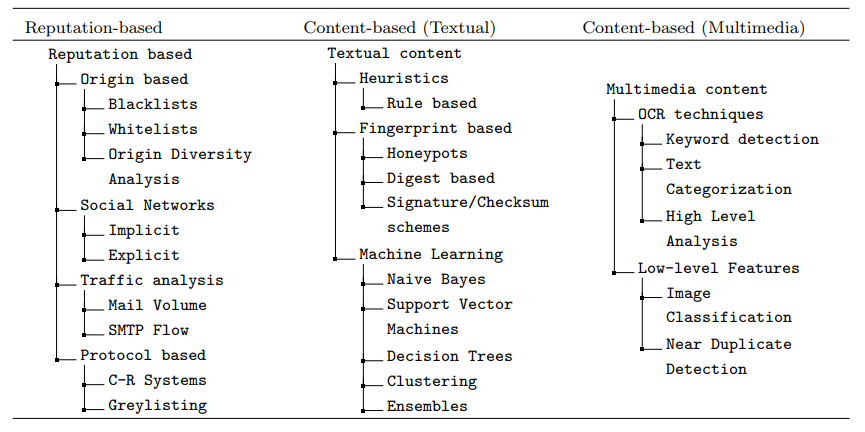
\includegraphics[scale=0.4]{classification.png}
\caption[]{Classification des méthodes}
\label{methodes}
\end{figure}
\end{center}

Ces méthodes sont surtout basées sur des techniques de Machine Learning et leurs variantes. Ce papier rend compte d'une analyse des idées pertinentes, des efforts, de l'efficacité des méthodes et des progrès actuels. Ce qui en ressort est que les recherches futures doivent aborder le fait que le filtrage du courrier indésirable est un problème qui évolue constamment, car à mesure que les nouveaux filtres tentent d'étendre les taux de prédiction, les spammeurs tentent de contrer les nouveaux algorithmes de prédiction en modifiant leur spams.\\Jusque là aucun filtre à spam n'a été capable d'assurer 100\% de chance de capture des spams et 0\% de chance d'obtention de faux spams.






\clearpage

\section{Références}

% solution provisoire en attendant que je fasse fonctionner bibli.bib

[1] Paul Graham, \textit{A plan for a spam}
, Août 2002, http://www.paulgraham.com/spam.html\\

[2] Paul Graham , \textit{Better Bayesian filtering}
, janvier 2003, http://www.paulgraham.com/better.html\\

[3] Alexy Bhowmick, Shyamanta M Hazarika , \textit{E-Mail Spam Filtering: A Review of Techniques and Trends}
, Janvier 2018 ,  https://www.researchgate.net/publication/320703241\_E-Mail\_Spam\_Filtering\_A\_Review\_of\_Techniques\_and\_Trends\\
%%\bibliographystyle{plain} % Le style est mis entre accolades.
%\bibliography{bibli}


\end{document}